% !TeX program = xelatex
\documentclass[UTF8,11pt,a4paper,linespread=1]{ctexart}
\usepackage[margin=26mm]{geometry}
\usepackage{amsmath,amssymb,bm}
\usepackage{setspace}
\setstretch{1.35}
\usepackage{pgfplots}
\pgfplotsset{compat=1.18}

\begin{document}
\section*{二参数模型的目标函数曲面}
\begin{center}
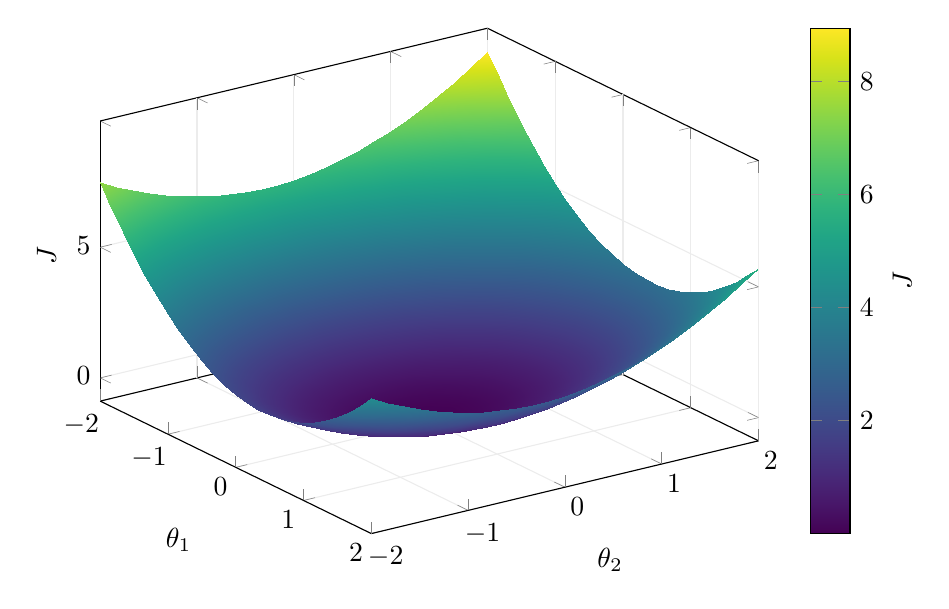
\begin{tikzpicture}
\begin{axis}[
  width=.82\linewidth,height=8cm,
  view={55}{30},
  xlabel={$\theta_1$},ylabel={$\theta_2$},zlabel={$J$},
  colormap/viridis,colorbar,
  colorbar style={ylabel={$J$}},
  grid=major,grid style={gray!15}
]
  % 这是示意目标函数，不是某次真实实验得到的误差面。
  \addplot3[
    surf,shader=interp,
    domain=-2:2,y domain=-2:2,
    samples=25,samples y=25
  ]{(x-.4)^2+.6*(y+.3)^2};
\end{axis}
\end{tikzpicture}
\end{center}
两个平方项同时为零时，函数取最小值 0，对应
\((\theta_1,\theta_2)=(0.4,-0.3)\)。图中的曲面由有限网格采样绘成。
\end{document}
